\section{Proposed solutions}

\begin{frame}{Multivariate outlier detection}

    Two \textbf{methods} are presented, both \textbf{based on the concept of multivariate outlier detection in the frequency domain}:

    \begin{itemize}
        \item Mahalanobis Square Distance (MSD)
        \item Principal Component Analysis (PCA)
    \end{itemize}

\end{frame}



\subsection{Mahalanobis Square Distance (MSD)}

\begin{frame}{Mahalanobis Square Distance (MSD) approach}

    The Mahalanobis Square Distance (MSD) is a measure of the distance between a point and a distribution. It is defined as:


    \begin{columns}[c, onlytextwidth]

        \begin{column}{0.5\textwidth}

            \begin{equation}
                D_{MSD}^2 = (\mathbf{x} - \mathbf{\mu})^T \mathbf{\Sigma}^{-1} (\mathbf{x} - \mathbf{\mu})
            \end{equation}

            Where:
            \begin{itemize}
                \item $\mathbf{x}_{(m \times 1)}$ is the vector of the observations
                \item $\mathbf{\mu}_{(m \times 1)}$ is the mean of the observations
                \item $\mathbf{\Sigma}_{(m \times m)}$ is the covariance matrix of the observations
            \end{itemize}

        \end{column}

        \hfill

        \begin{column}{0.45\textwidth}

            \begin{figure}[H]
                \centering
                % https://it.mathworks.com/help/stats/mahal.html
                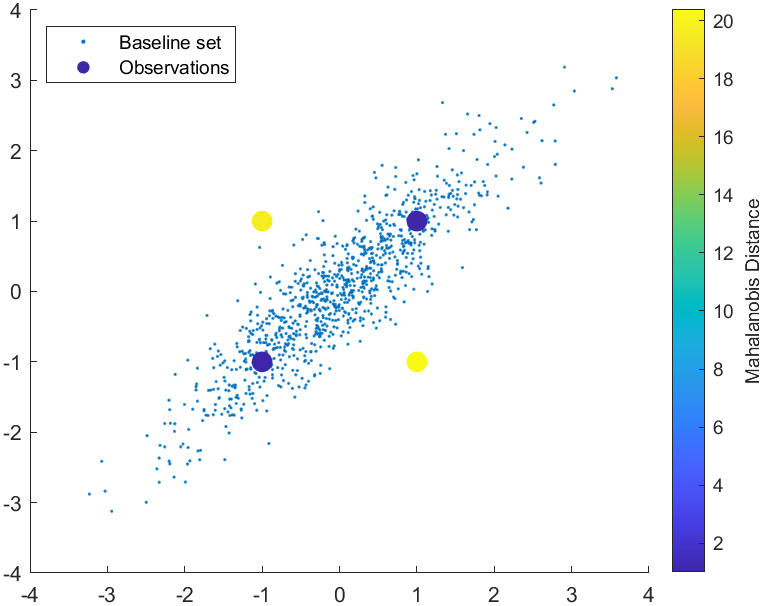
\includegraphics[width=\textwidth]{img/Mahalanobis-cloud-plot.png}
                \caption{Application example of the MSD index. \textcolor[HTML]{F5EC22}{Outliers} are clearly visible.}
            \end{figure}

        \end{column}

    \end{columns}

    \vspace{9pt}

    The MSD is used to detect outliers in the data, by comparing the distance of each observation from the mean of the distribution.

\end{frame}



\begin{frame}{Problematic of the MSD approach}

    The MSD approach is \textbf{based on the assumption that the baseline data contains all the possible variations due to environmental effects} (e.g. temperature, vibrations noise, etc.).

    \vspace{9pt}

    To be effective then, the baseline data should be collected in a wide range of environmental conditions, in order to capture all the possible variations, \textbf{which imply a long and expensive data collection campaign} that is not always feasible.

\end{frame}



\subsection{Principal Component Analysis (PCA)}

\begin{frame}{Principal Component Analysis (PCA) approach}

    The Principal Component Analysis (PCA) is a statistical method used to project the data onto a new coordinate system, where the new axes are the principal components of the data.

    % https://builtin.com/data-science/step-step-explanation-principal-component-analysis
    \begin{figure}[H]
        \centering
        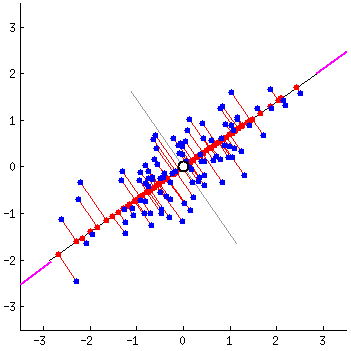
\includegraphics[width=0.3\textwidth]{img/principal-components-01.png}
        \hfill
        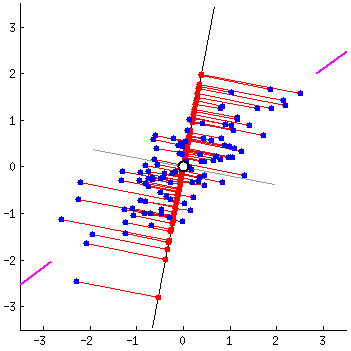
\includegraphics[width=0.3\textwidth]{img/principal-components-02.png}
        \hfill
        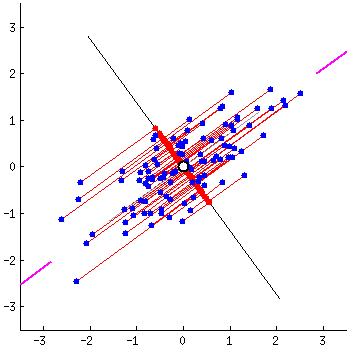
\includegraphics[width=0.3\textwidth]{img/principal-components-03.png}
        \caption{Example of PCA applied to a 2D dataset. Minimums of the distance function between the points and the set of new axes, determines the principal components. With refer to the figures, $1^{st}$ and $3^{rd}$ represent two different PCs configurations, while the $2^{nd}$ mimics the rotational transformation of the data.}
    \end{figure}

    In a broad, the result of the PCA can be interpreted ad the `eigenvectors' of the cloud of data.

\end{frame}



\begin{frame}{Singular Value Decomposition (SVD) in the PCA approach}

    In order to perform the PCA, a rotational transformation of the data is needed (i.e. the data is rotated in order to find the principal components).

    The Singular Value Decomposition (SVD) is a mathematical technique used to compute this transformation.

    By definition, SVD of a matrix $\mathbf{A}$ is defined as:

    \begin{equation}
        \mathbf{A} = \mathbf{U} \mathbf{\Sigma} \mathbf{V}^T
    \end{equation}

    Where:
    \begin{itemize}
        \item $\mathbf{U}$ is the matrix of the left singular vectors of $\mathbf{A}$
        \item $\mathbf{\Sigma}$ is the diagonal matrix of the singular values of $\mathbf{A}$
        \item $\mathbf{V}$ is the matrix of the right singular vectors of $\mathbf{A}$
    \end{itemize}



\end{frame}



\begin{frame}{Analysis of signals via PCA}

    Given that just the first(s) principal component(s) are affected by environmental conditions, we can think of remove them from the data and apply the MSD approach to detect outliers of this dimensionally reduced dataset.

    \begin{figure}
        \centering
        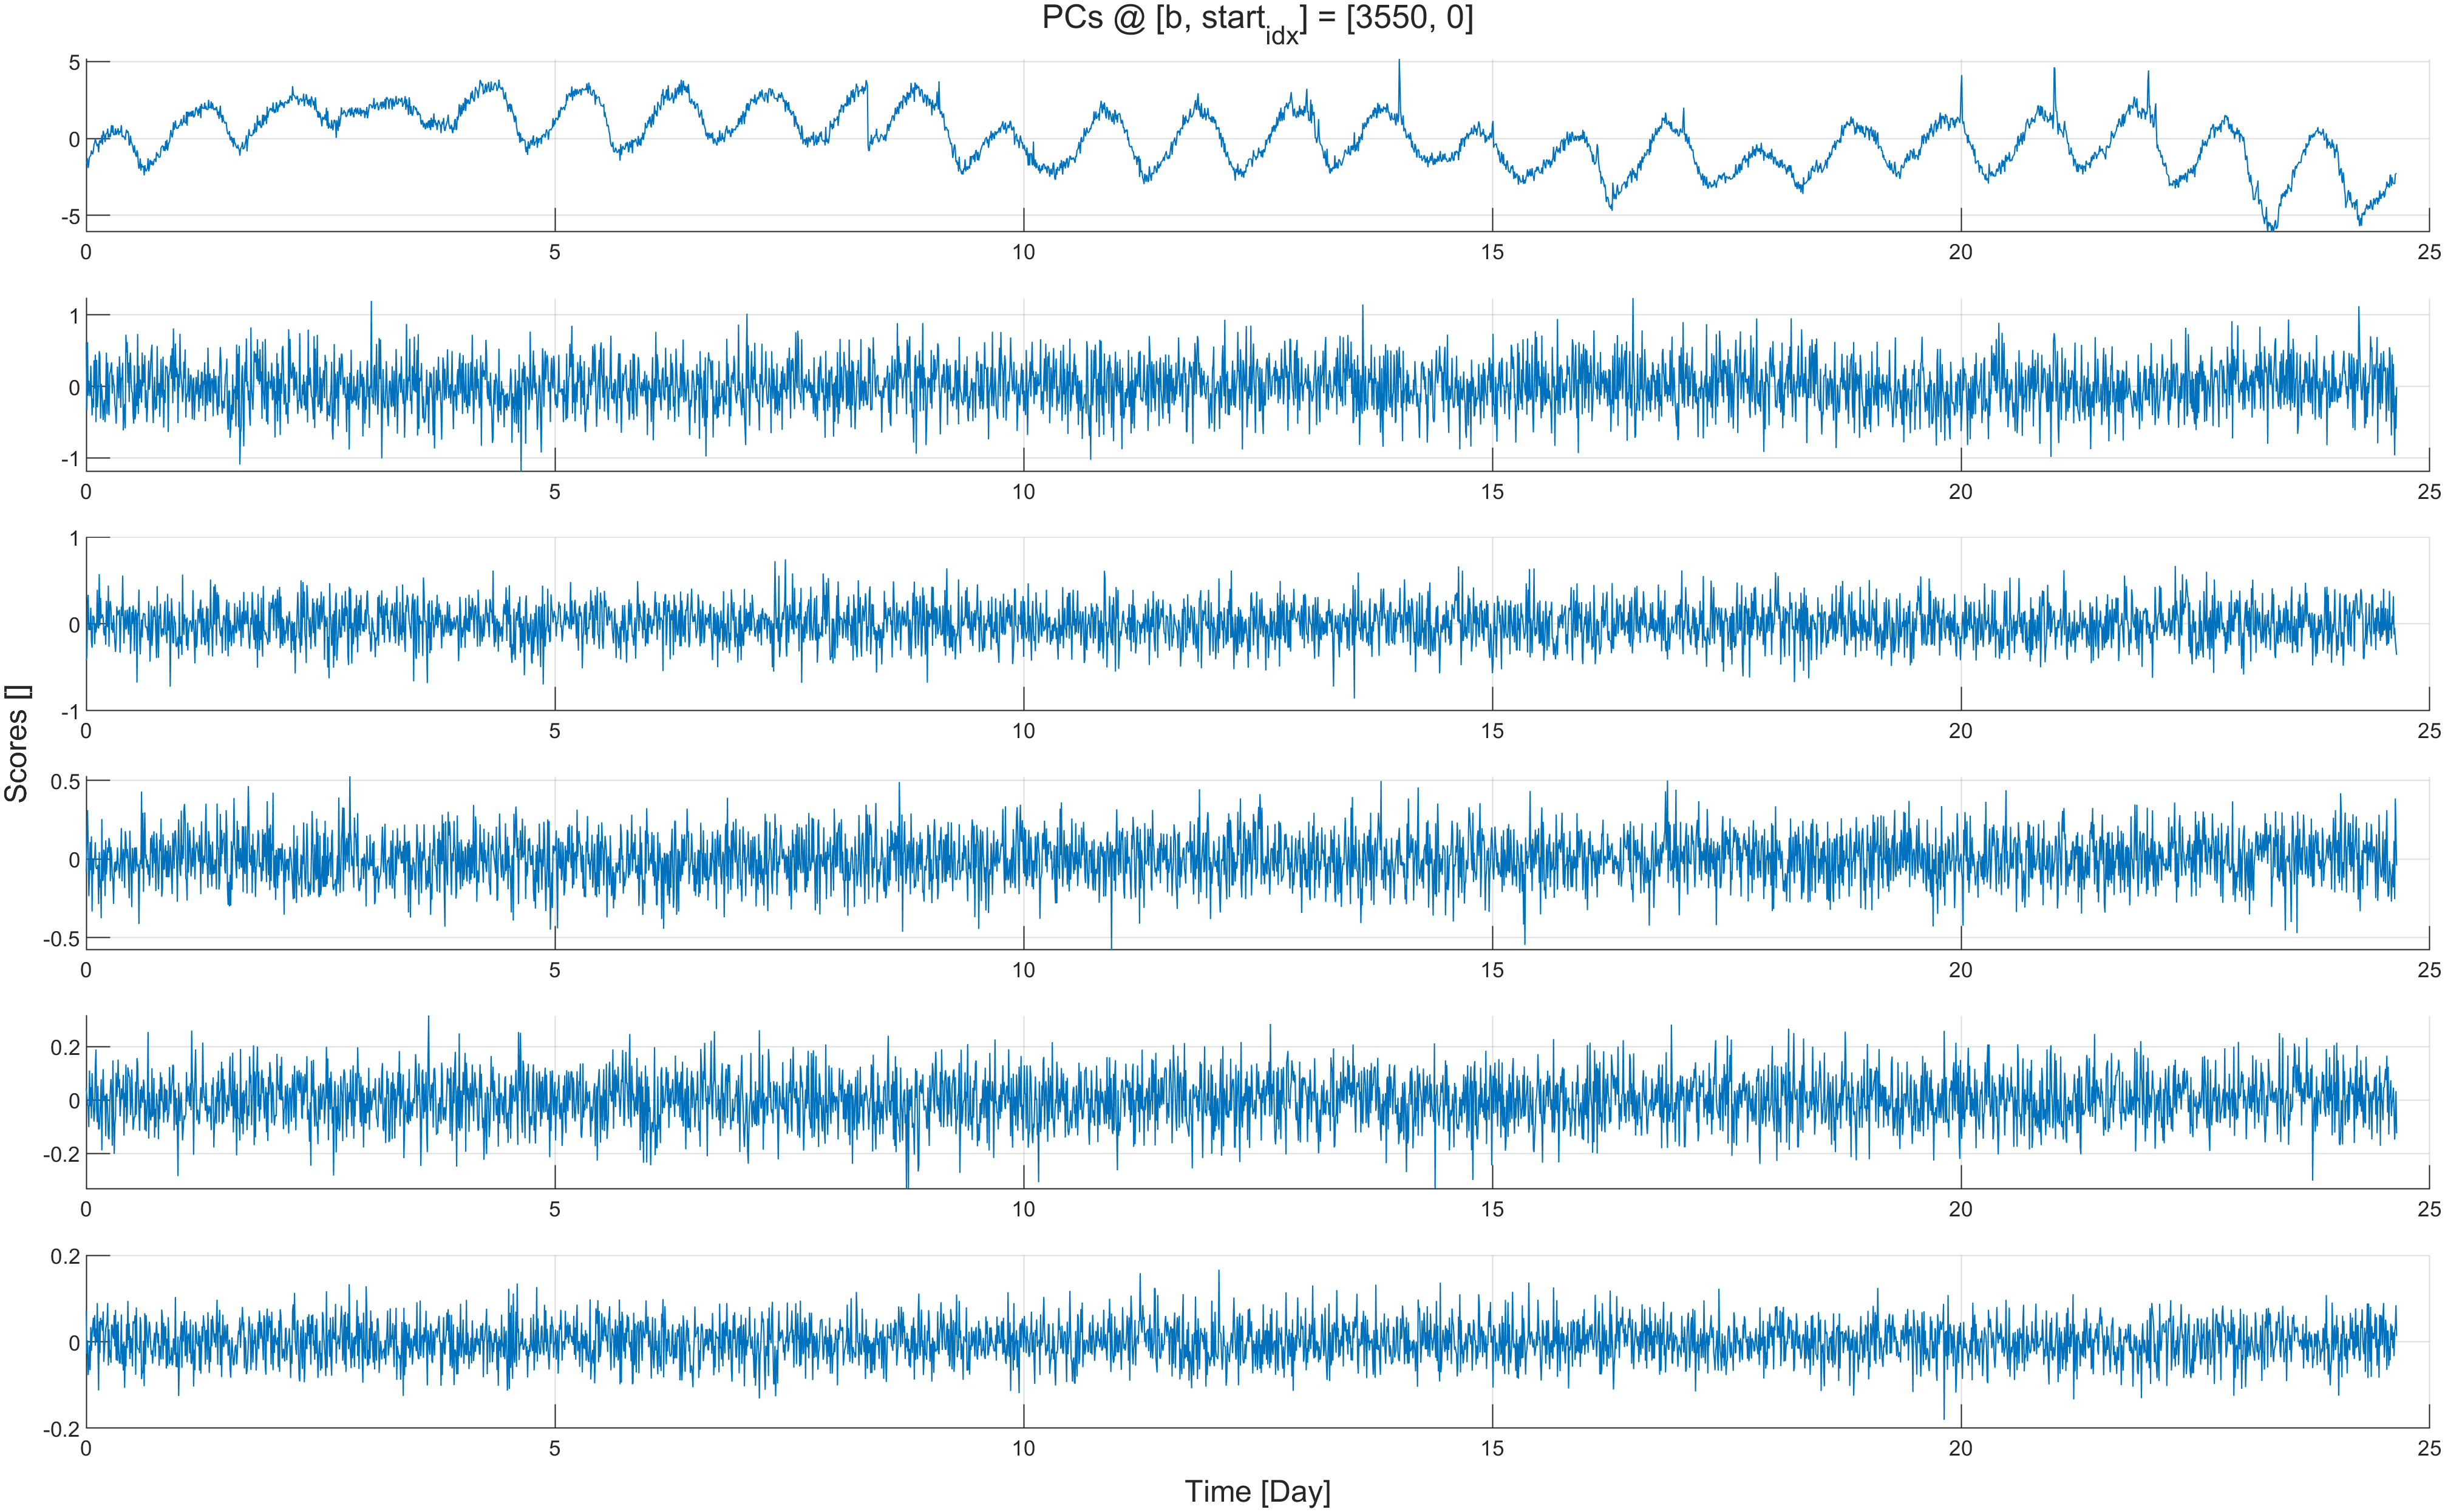
\includegraphics[width=0.9\textwidth]{img/MATLAB/PCs_01.png}
        \caption{Scores of the eigenfrequencies of the structure projected into the principal components. Notice the clear decreasing trend of the deterministic amount as we consider higher principal components. Here, $b = 20\% \times data_{sampled} = 3550$.}
    \end{figure}

\end{frame}